\section{Expected Performance of Tau Identification with RNN}%
\label{sec:tauid_perf}

Thresholds on the RNN scores of 1- and 3-prong \tauhadvis candidates define
working points of varying \tauhadvis identification efficiencies and
\faketauhadvis rejection factors.\footnote{The \tauhadvis identification
  efficiency is the fraction of \truetauhadvis from simulated
  $\gammastar \to \tautau$ events that pass a given working point. The
  \faketauhadvis rejection is the reciprocal of the fraction of \faketauhadvis
  from simulated dijet events that pass a given working point.} Four named
working points are defined to cover the needs of most physics analyses at the
ATLAS experiment. These working points are, in order of increasing
\faketauhadvis rejection: \emph{very loose}, \emph{loose}, \emph{medium}, and
\emph{tight}.

The targeted \tauhadvis identification efficiencies of the working points are
summarised in \Cref{tab:rnn_wps}. The rejection of \faketauhadvis from simulated
dijet events is compared between the BDT- and RNN-based \tauid algorithms for
working points targeting the same \tauhadvis efficiency. The RNN \tauid improves
the \faketauhadvis rejection by about \SI{80}{\percent} for 1-prong and between
\SIrange{40}{80}{\percent} for 3-prong \tauhadvis candidates over the BDT-based
method. The majority of these improvements stem from the inclusion of
charge-particle track information in addition to the high-level variables also
used in the BDT. The receiver operating characteristic curves of both algorithms
are shown in \Cref{fig:tauid_rnn_bdt_roc_comparison}.

\begin{table}[htbp]
  \centering

  \caption[Comparison of working points defined for the BDT and RNN-based
  \tauid.]{Comparison of working points defined for the BDT and RNN-based
    \tauid. Only the targeted \tauhadvis efficiency (target \tauhadvis eff.) of
    the working points is given which can deviate by ca.\ \SI{1}{\percent} from
    the actual efficiency observed in simulated $\gammastar \to \tautau$
    events. The \faketauhadvis rejection is evaluated using the \tauhadvis
    candidate sample from dijet events. The table is adapted from
    Ref.~\cite{ATL-PHYS-PUB-2019-033}.}%
  \label{tab:rnn_wps}

  \begin{tabular}{l
  cc
  @{\hskip 20pt}
  S[table-format=3.1]S[table-format=3.1]
  @{\hskip 20pt}
  S[table-format=3.1]S[table-format=3.1]}
  \toprule
  Working point & \multicolumn{2}{c@{\hskip 20pt}}{Signal efficiency} & \multicolumn{4}{c}{Background rejection} \\
  \cmidrule{4-7}
  &&& \multicolumn{2}{c@{\hskip 20pt}}{BDT} & \multicolumn{2}{c}{RNN} \\
                 & {1-prong} & {3-prong} & {1-prong} & {3-prong} & {1-prong} & {3-prong} \\
  \midrule
  Tight          & 60\,\%    & 45\,\%    & 40      & 420  & 72   & 770 \\
  Medium         & 75\,\%    & 60\,\%    & 20      & 160  & 36   & 260 \\
  Loose          & 85\,\%    & 75\,\%    & 12      & 66   & 21   & 99  \\
  Very loose     & 95\,\%    & 95\,\%    & 5.4     & 12   & 10   & 17  \\
  \bottomrule
\end{tabular}

% RNN tight 1P (rej): (71.96561246250148, 1.5303654439176062)
% RNN tight 1P (eff): (0.6117071909689276, 0.00024632688674175375)

% RNN tight 3P (rej): (773.933684779941, 39.28717816847519)
% RNN tight 3P (eff): (0.4566744467549334, 0.0003930521163405298)

% RNN medium 1P (rej): (35.82174458925124, 0.5877811653533531)
% RNN medium 1P (eff): (0.7597229941852967, 0.00028684295761911014)

% RNN medium 3P (rej): (264.41485204506034, 8.335133701736764)
% RNN medium 3P (eff): (0.6070290461673806, 0.00047597265519827683)

% RNN loose 1P (rej): (21.451007928217003, 0.2689671234302654)
% RNN loose 1P (eff): (0.8571601779651077, 0.00031300330970361357)

% RNN loose 3P (rej): (98.88497042998625, 1.8186512443248162)
% RNN loose 3P (eff): (0.756200706125848, 0.0005553554612403042)

% RNN veryloose 1P (rej): (10.059399296744843, 0.08444372648580398)
% RNN veryloose 1P (eff): (0.953066083106346, 0.0003384639200436791)

% RNN veryloose 3P (rej): (17.088578294479646, 0.13369860249913534)
% RNN veryloose 3P (eff): (0.9521385218793144, 0.0006570081893723098)

% BDT tight 1P (rej): (40.45967058185579, 0.7041781103272695)
% BDT tight 1P (eff): (0.5979792716851993, 0.00024250506003222104)

% BDT tight 3P (rej): (417.43136176200227, 16.77018703333453)
% BDT tight 3P (eff): (0.44928881105722246, 0.0003888705286576926)

% BDT medium 1P (rej): (20.35364225713967, 0.24775946939663773)
% BDT medium 1P (eff): (0.7493892746348453, 0.00028404624937242954)

% BDT medium 3P (rej): (159.3582135014997, 3.9403189472371616)
% BDT medium 3P (eff): (0.5996076427209064, 0.0004719599960117791)

% BDT loose 1P (rej): (11.788490308526693, 0.10777438892574735)
% BDT loose 1P (eff): (0.850531538104052, 0.000311232976426111)

% BDT loose 3P (rej): (65.58988709376405, 0.978622556721974)
% BDT loose 3P (eff): (0.7517812018543497, 0.0005530325740489808)

% BDT veryloose 1P (rej): (5.423518802654415, 0.03531494188085259)
% BDT veryloose 1P (eff): (0.9508788348923811, 0.00033788569007909387)

% BDT veryloose 3P (rej): (12.100080401977765, 0.08023605419699714)
% BDT veryloose 3P (eff): (0.9511017578180401, 0.0006564758961708566)

%%% Local Variables:
%%% mode: latex
%%% TeX-master: "../phd_thesis"
%%% End:

\end{table}

\begin{figure}[htbp]
  \centering

  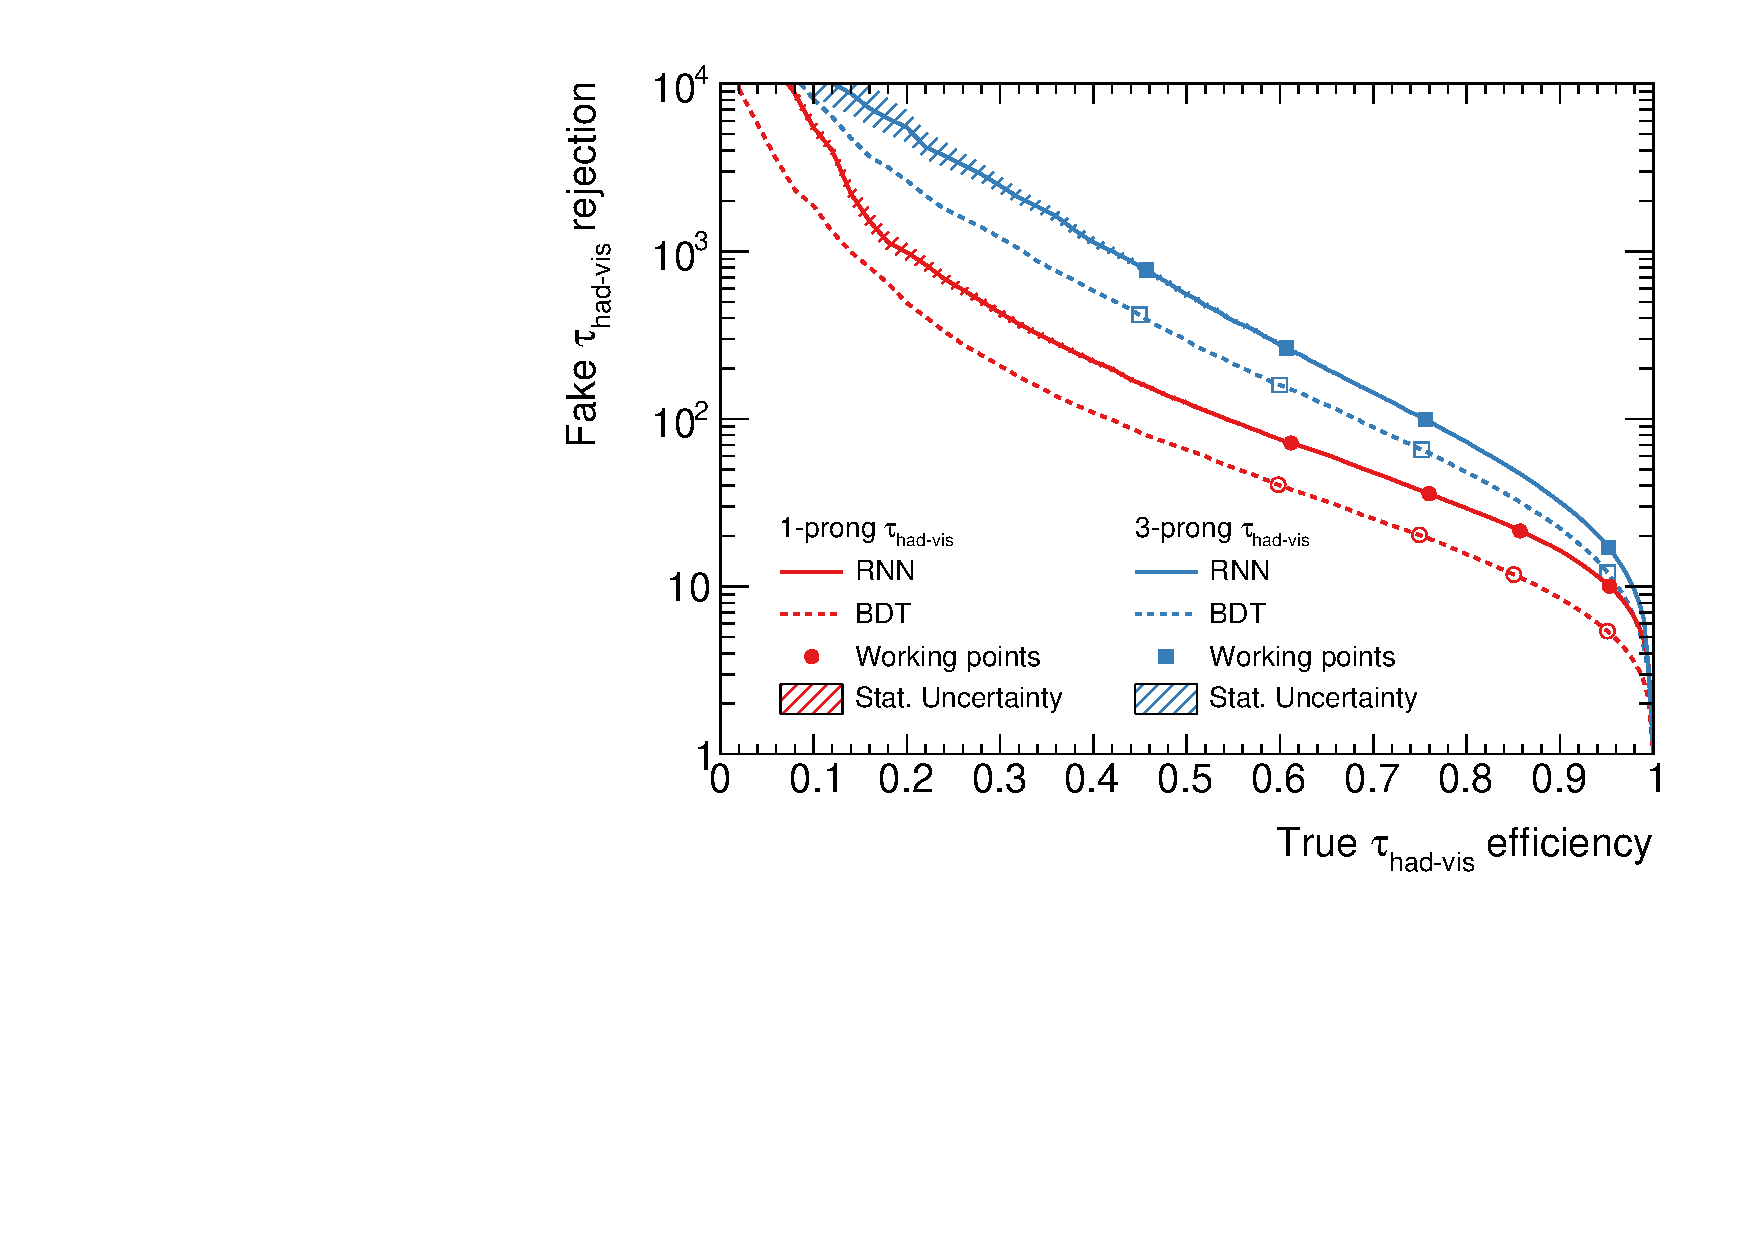
\includegraphics[width=0.55\textwidth]{tauid/roc_incl_witherrors}

  \caption[Receiver operating characteristic curve of the \tauid algorithms
  based on RNN and BDT.]{Receiver operating characteristic curve of the \tauid
    algorithms based on RNN (solid) and BDT (dashed) shown separately for 1-
    (red) and 3-prong (blue) candidates. The true- and \faketauhadvis
    efficiencies are evaluated using samples of \tauhadvis candidates from
    $\gammastar \to \tautau$ and dijet events, respectively.  The figure is
    adapted from Ref.~\cite{ATL-PHYS-PUB-2019-033}.}%
  \label{fig:tauid_rnn_bdt_roc_comparison}
\end{figure}

The \tauhadvis identification efficiencies
% estimated using \tauhadvis from simulated $\gammastar \to \tautau$ events
are shown in \Cref{fig:tauid_truetau_eff} for all four working points in bins of
\tauhadvis \pT, \tauhadvis $|\eta|$, and the average number of interactions per
bunch crossing, $\mu$. The efficiency remains approximately constant as
\tauhadvis \pT and $\mu$ is varied due to the definition of the working points
using the transformed output of the neural network. An exception is the first
\tauhadvis \pT bin which does not meet the target efficiency. This is an effect
of different \tauhadvis momentum calibrations being used for the transformation
of the RNN output and for the performance evaluation shown in
\Cref{fig:tauid_truetau_eff_a,fig:tauid_truetau_eff_b}. The transformation was
derived using the calorimeter-based \tauhadvis \pT estimate at LC scale, which
is now superseded by a multivariate method combining information from the
calorimeters and tracking systems (shown in the figures).

\begin{figure}[htbp]

  \begin{subfigure}{0.498\textwidth}
    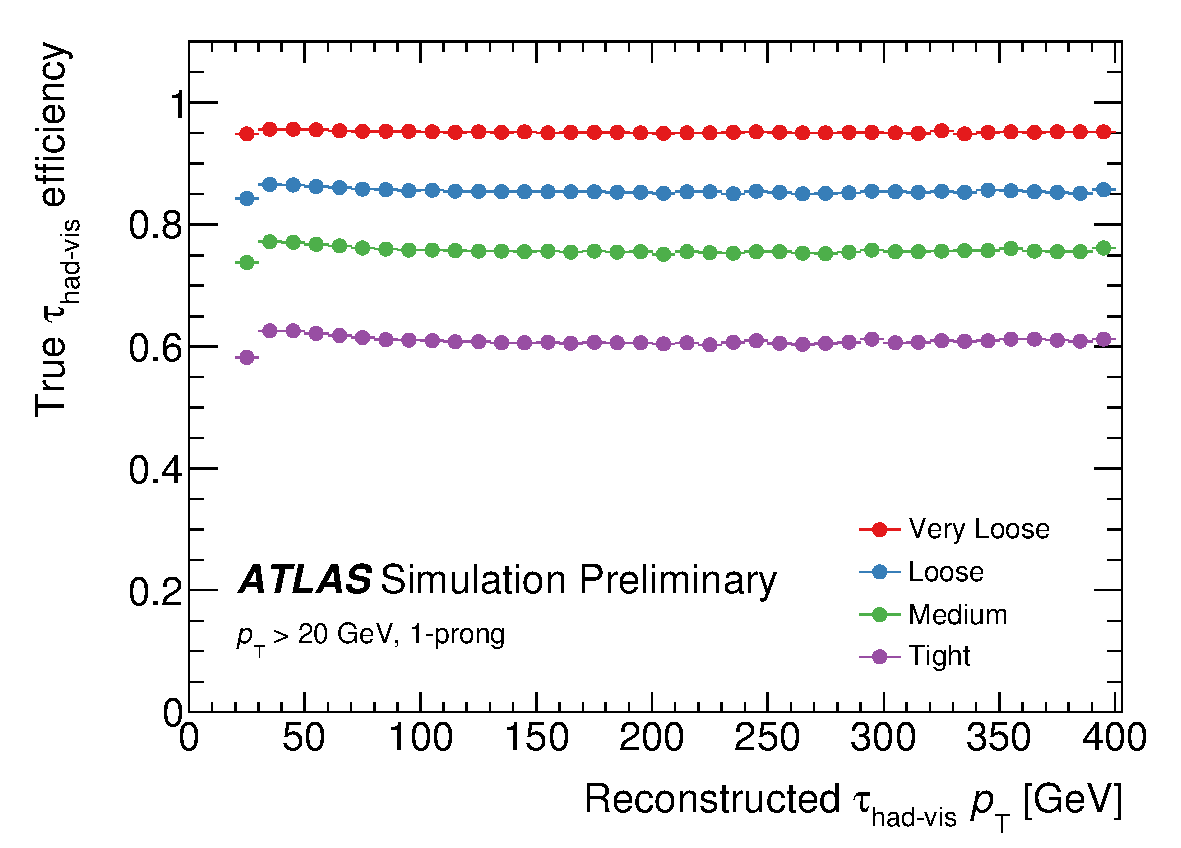
\includegraphics[width=\textwidth]{tauid/pubnote/eff_vs_pt_1p}
    \subcaption{}%
    \label{fig:tauid_truetau_eff_a}
  \end{subfigure}\hfill%
  \begin{subfigure}{0.498\textwidth}
    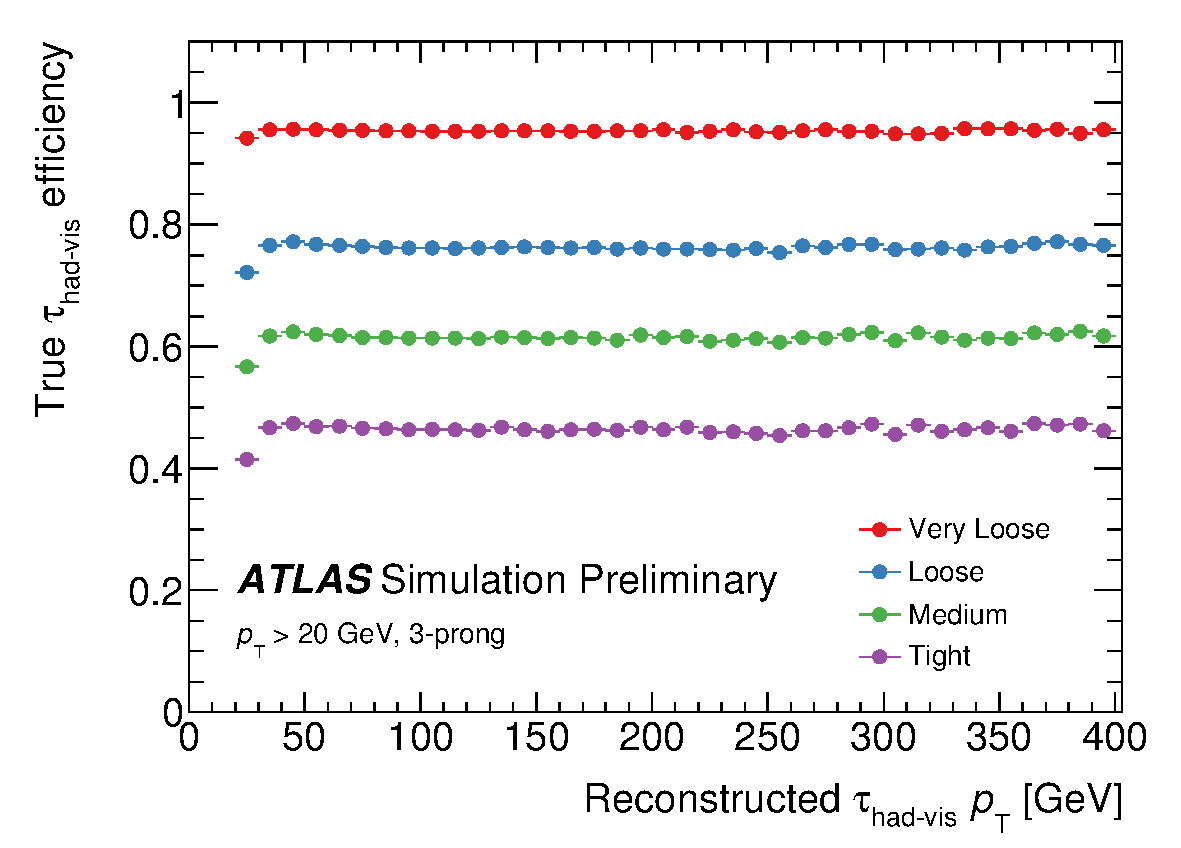
\includegraphics[width=\textwidth]{tauid/pubnote/eff_vs_pt_3p}
    \subcaption{}%
    \label{fig:tauid_truetau_eff_b}
  \end{subfigure}

  \begin{subfigure}{0.498\textwidth}
    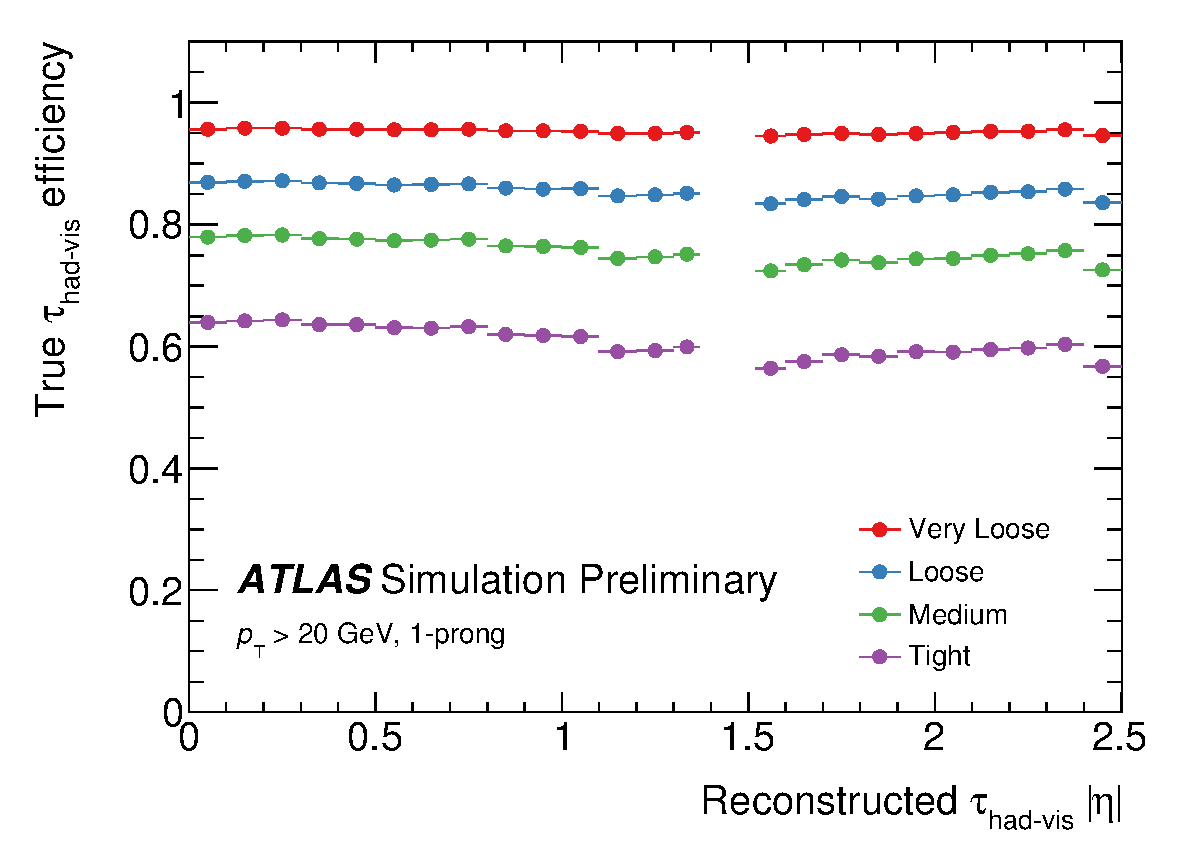
\includegraphics[width=\textwidth]{tauid/pubnote/eff_vs_eta_1p}
    \subcaption{}
  \end{subfigure}\hfill%
  \begin{subfigure}{0.498\textwidth}
    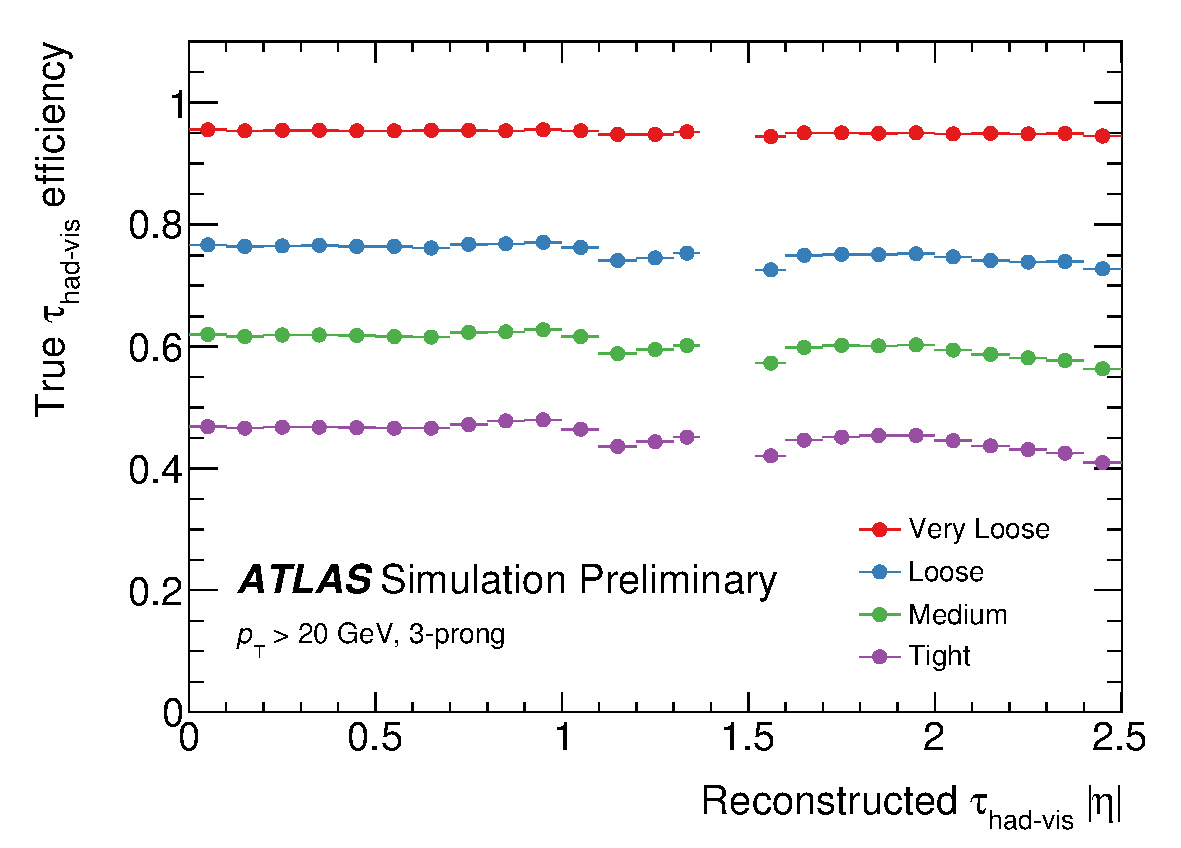
\includegraphics[width=\textwidth]{tauid/pubnote/eff_vs_eta_3p}
    \subcaption{}
  \end{subfigure}

  \begin{subfigure}{0.498\textwidth}
    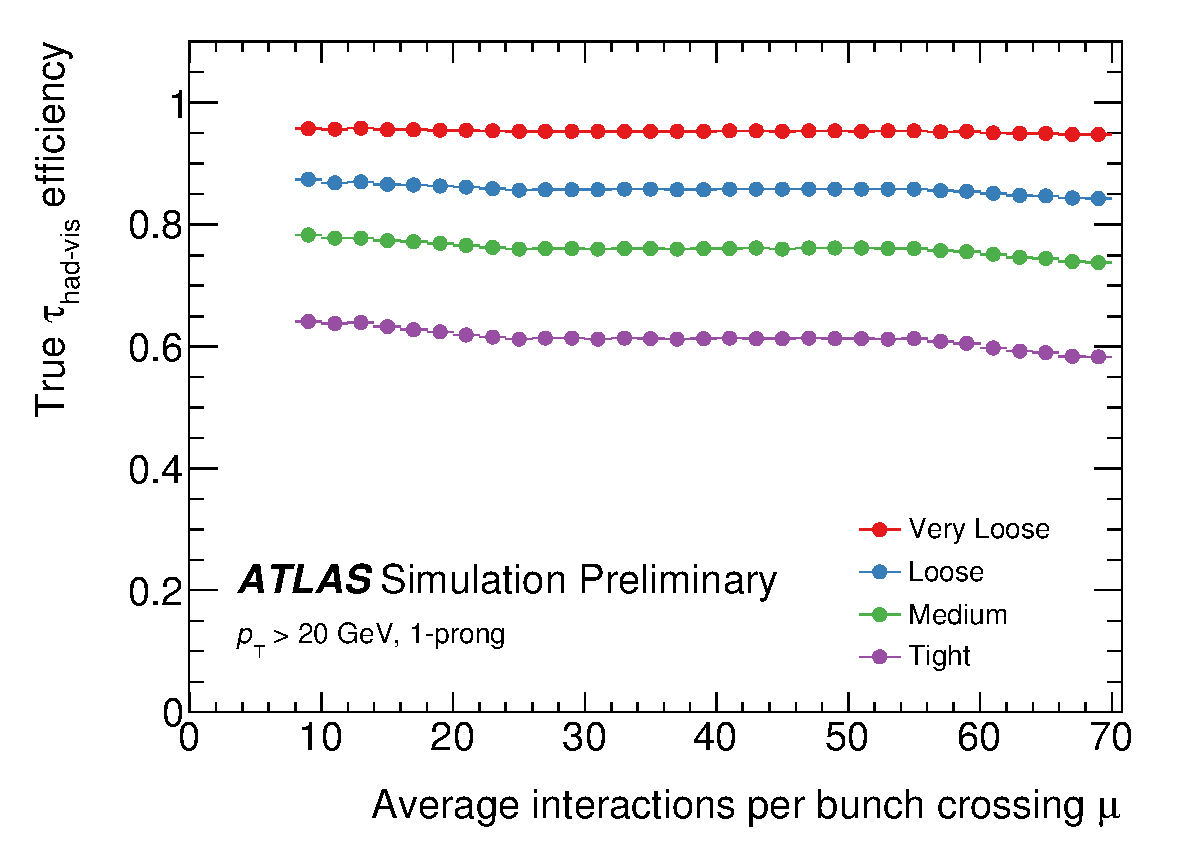
\includegraphics[width=\textwidth]{tauid/pubnote/eff_vs_mu_1p}
    \subcaption{}
  \end{subfigure}\hfill%
  \begin{subfigure}{0.498\textwidth}
    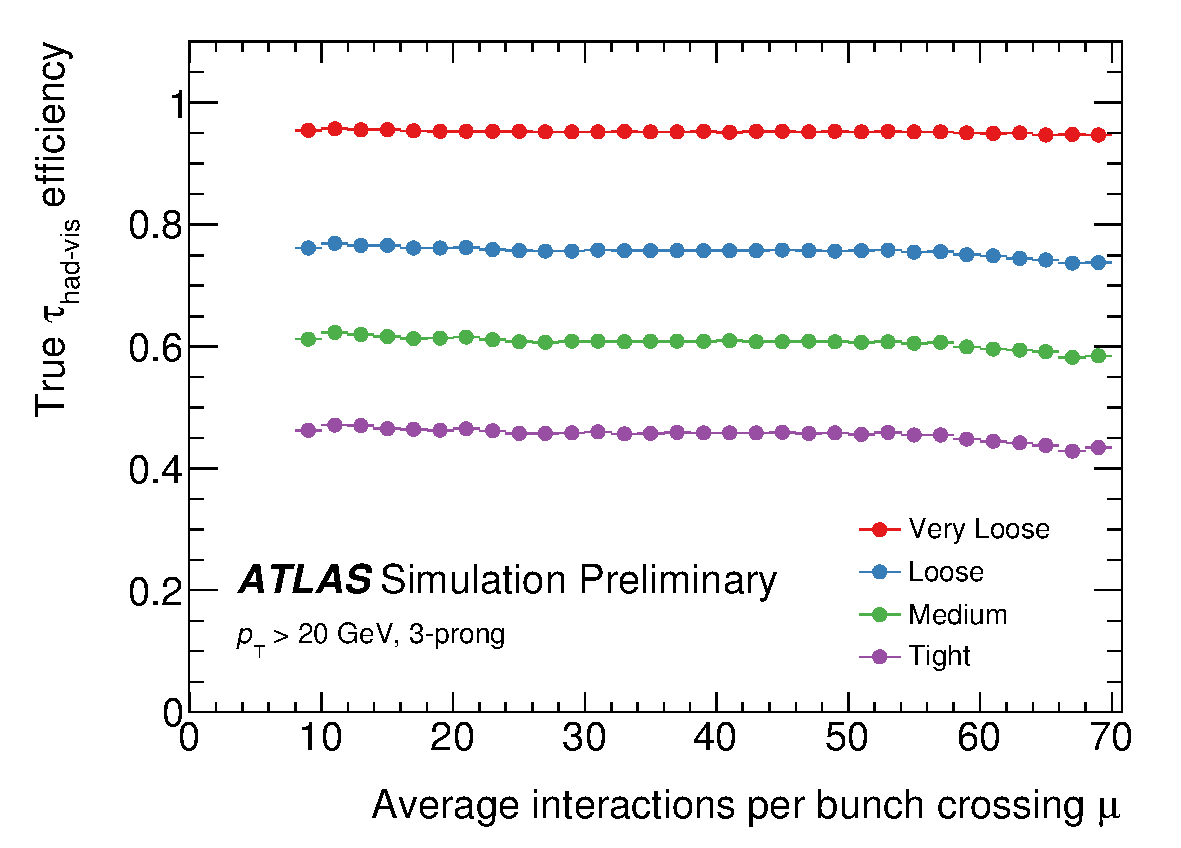
\includegraphics[width=\textwidth]{tauid/pubnote/eff_vs_mu_3p}
    \subcaption{}
  \end{subfigure}

  \caption[True-\tauhadvis efficiencies of the RNN \tauid working
  points.]{True-\tauhadvis efficiencies of the RNN \tauid working points. The
    efficiencies are estimated using \tauhadvis candidates from simulated
    $\gammastar \to \tautau$ events separately for 1- (left) and 3-prong (right)
    \tauhadvis. Efficiencies are shown in bins of \tauhadvis \pT (top),
    \tauhadvis $|\eta|$ (middle), and the average number of interactions per
    bunch crossing (bottom). All figures are taken from
    Ref.~\cite{ATL-PHYS-PUB-2019-033}.}%
  \label{fig:tauid_truetau_eff}
\end{figure}

The rejection of \faketauhadvis from simulated dijet events by the \emph{medium}
\tauid working points of the BDT- and RNN-based methods is compared
in~\Cref{fig:tauid_faketau_rej}. The comparison is performed separately for 1-
and 3-prong \tauhadvis candidates and in bins of \tauhadvis \pT, \tauhadvis
$|\eta|$, and $\mu$. In general, the \faketauhadvis rejection of \tauid is
analysis and process dependent\footnote{The ratio of quark- to gluon-initiated
  jets affects the \faketauhadvis rejection since gluon-initiated jets are more
  easily rejected by \tauid. Additionally, the rejection depends on the \pT and
  \Ntracks of \faketauhadvis and thus on the selections applied by analyses.}
and thus the comparison mainly serves as a benchmark of the identification
algorithms.

The \faketauhadvis rejection of \tauid increases with \tauhadvis
candidate \pT as is shown in
\Cref{fig:tauid_faketau_rej_a,fig:tauid_faketau_rej_b}. This trend is
partially explained by the increasing discrimination power of
variables sensitive to the isolation of \tauhadvis candidates as
larger momentum scales are considered. This is a consequence of the
increasing collimation of \truetauhadvis due to the Lorentz boost of
the \taulepton while \faketauhadvis become less isolated due to the
increase in the average charged and neutral hadron multiplicity in
jets.

% Improved discrimination power is also expected for variables
% sensitive to the \taulepton lifetime for 3-prong \tauhadvis where
% the secondary vertex will, on average, have a larger displacement
% from the PV.

The RNN \tauid improves the \faketauhadvis rejection by a factor of
two for 1- and 3-prong \tauhadvis candidates with
$\pT > \SI{70}{\GeV}$ over the BDT-based approach at comparable
working points. Similar behaviour of the \faketauhadvis rejection is
observed for both methods with respect to the pseudorapidity of
\tauhadvis candidates. However, the RNN \tauid is more susceptible to
pile-up compared to the BDT-based method. This is depicted
in~\Cref{fig:tauid_faketau_rej_e,fig:tauid_faketau_rej_f} showing a
degradation in \faketauhadvis rejection as the average number of
interactions per bunch crossing increases.

\begin{figure}[htbp]

  \begin{subfigure}{0.498\textwidth}
    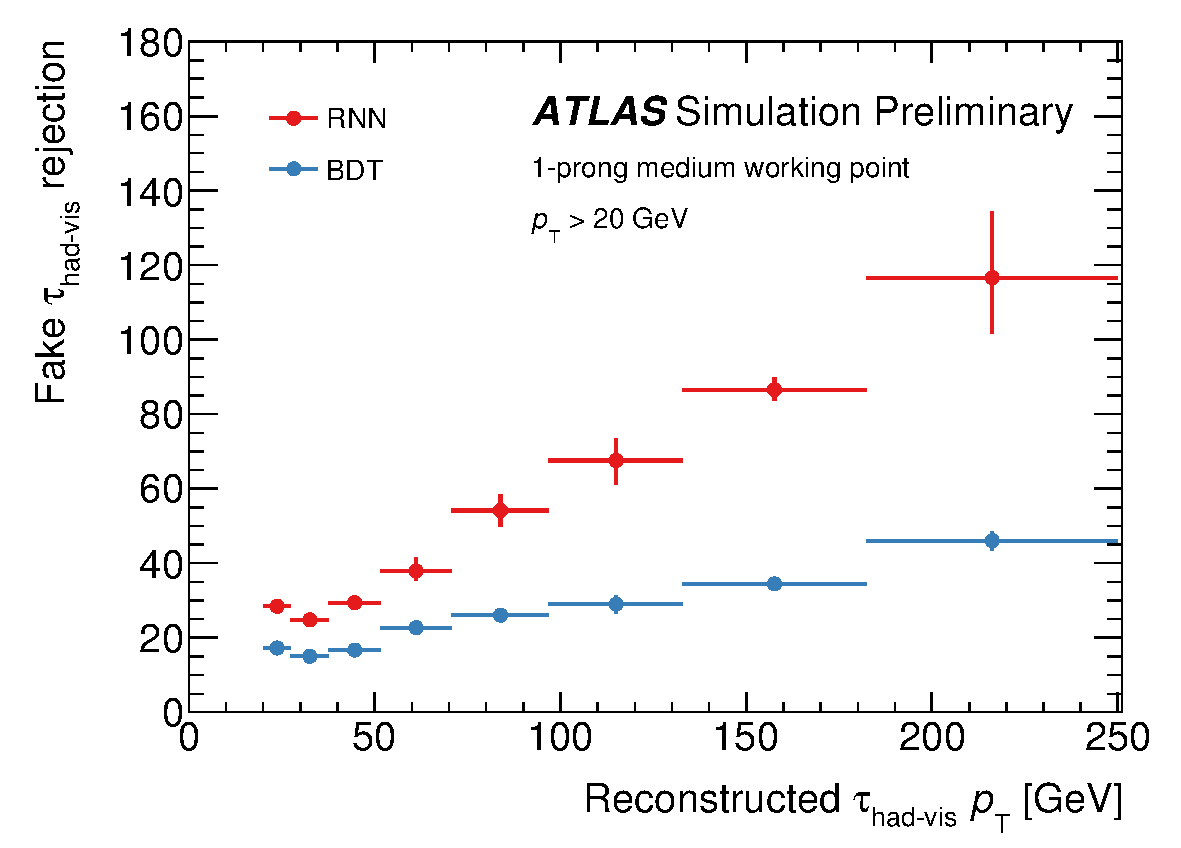
\includegraphics[width=\textwidth]{tauid/pubnote/rej_vs_pt_1p}
    \subcaption{}%
    \label{fig:tauid_faketau_rej_a}
  \end{subfigure}\hfill%
  \begin{subfigure}{0.498\textwidth}
    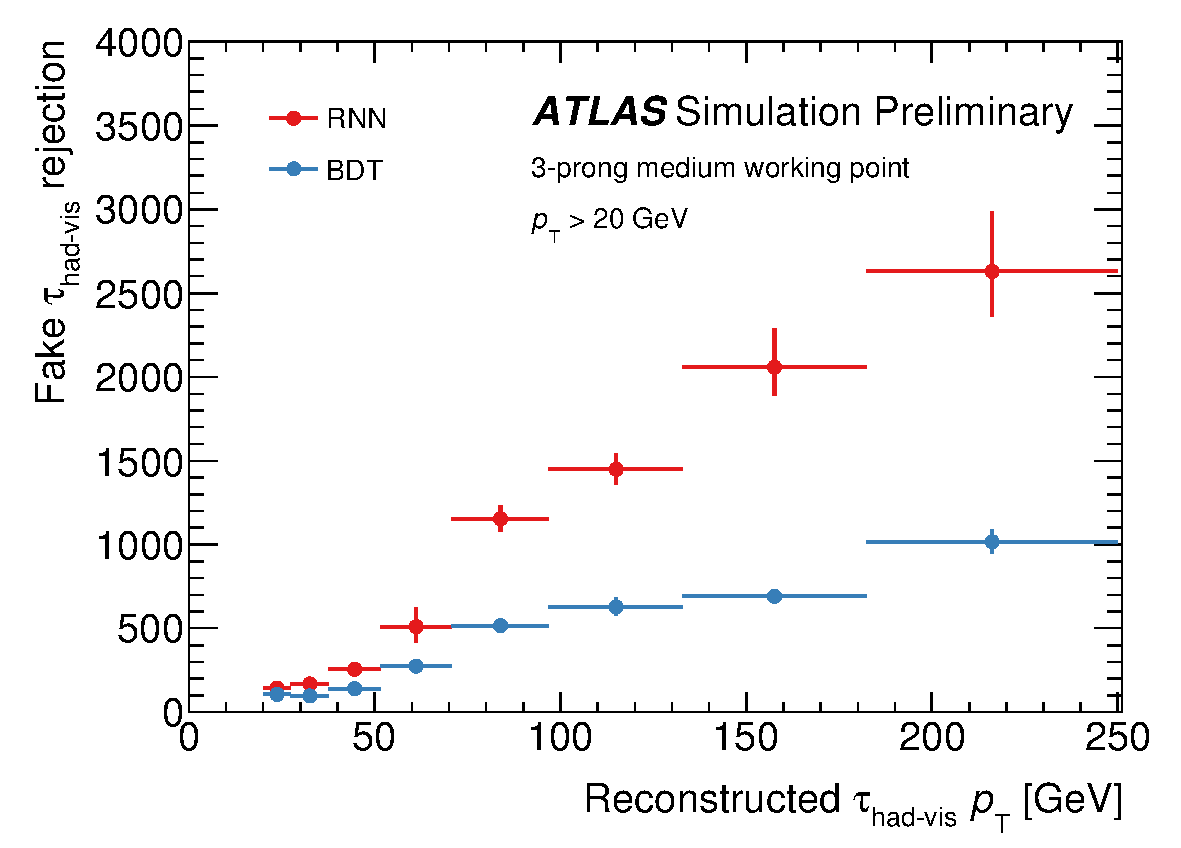
\includegraphics[width=\textwidth]{tauid/pubnote/rej_vs_pt_3p}
    \subcaption{}%
    \label{fig:tauid_faketau_rej_b}
  \end{subfigure}

  \begin{subfigure}{0.498\textwidth}
    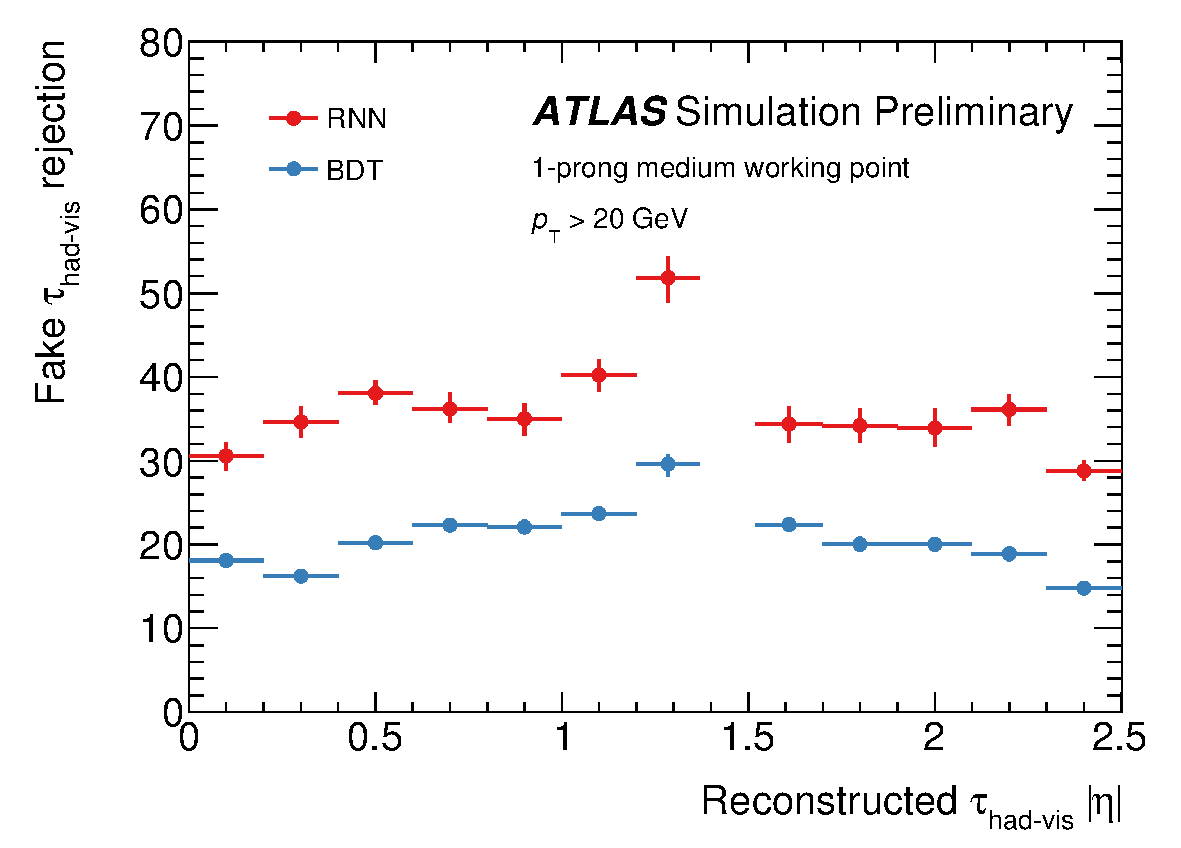
\includegraphics[width=\textwidth]{tauid/pubnote/rej_vs_eta_1p}
    \subcaption{}
  \end{subfigure}\hfill%
  \begin{subfigure}{0.498\textwidth}
    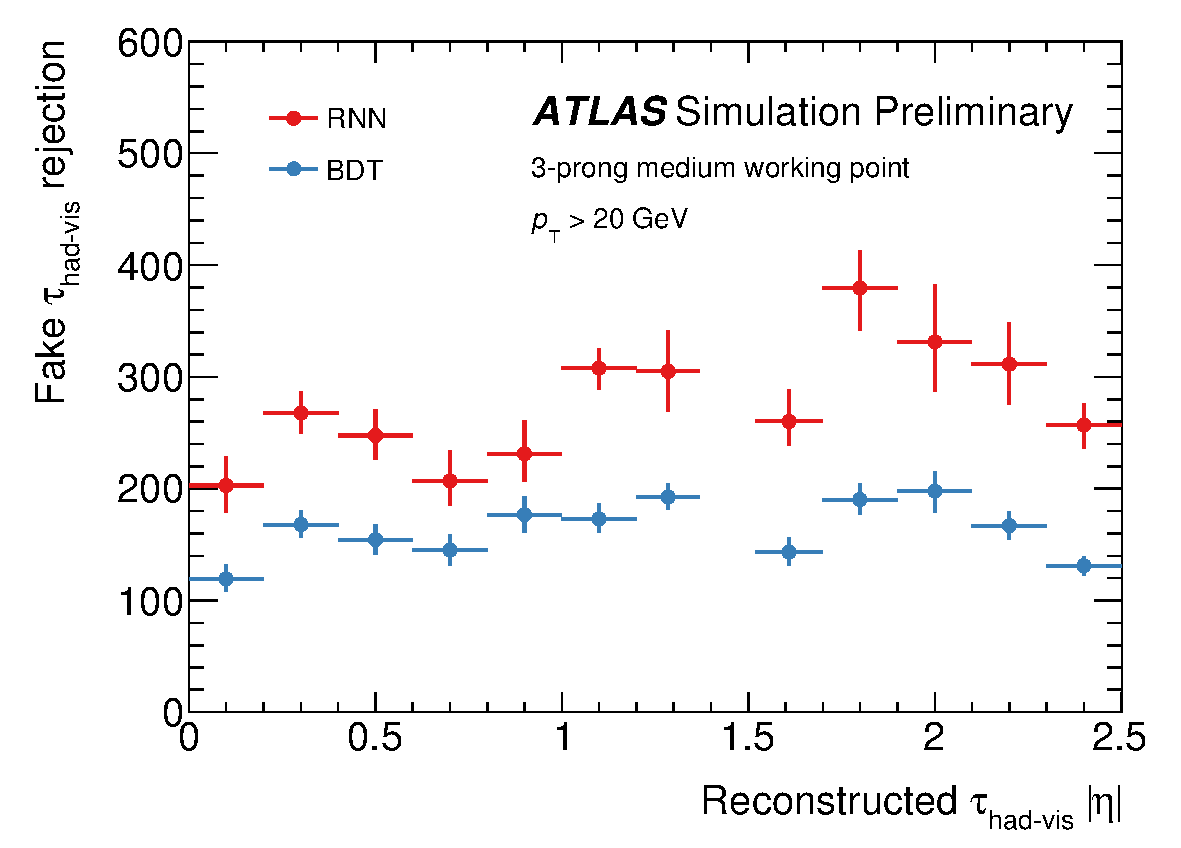
\includegraphics[width=\textwidth]{tauid/pubnote/rej_vs_eta_3p}
    \subcaption{}
  \end{subfigure}

  \begin{subfigure}{0.498\textwidth}
    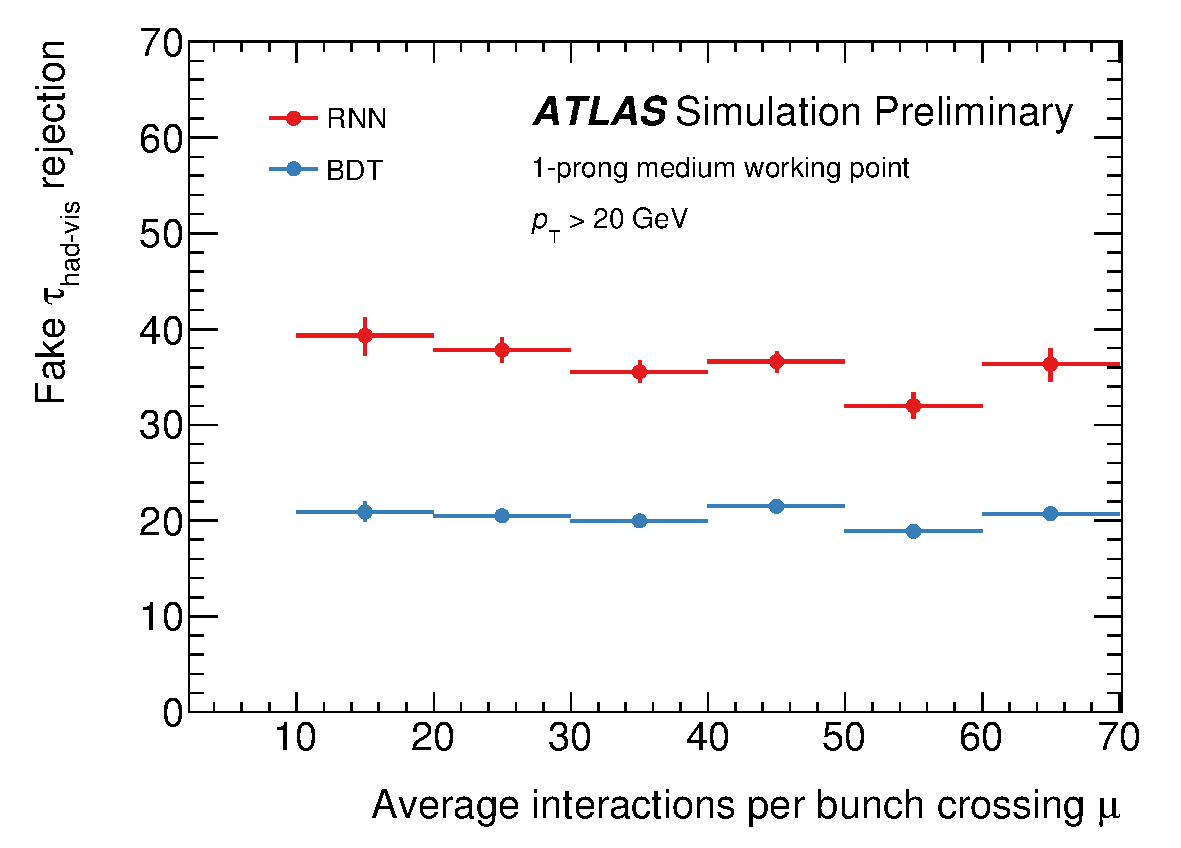
\includegraphics[width=\textwidth]{tauid/pubnote/rej_vs_mu_1p}
    \subcaption{}%
    \label{fig:tauid_faketau_rej_e}
  \end{subfigure}\hfill%
  \begin{subfigure}{0.498\textwidth}
    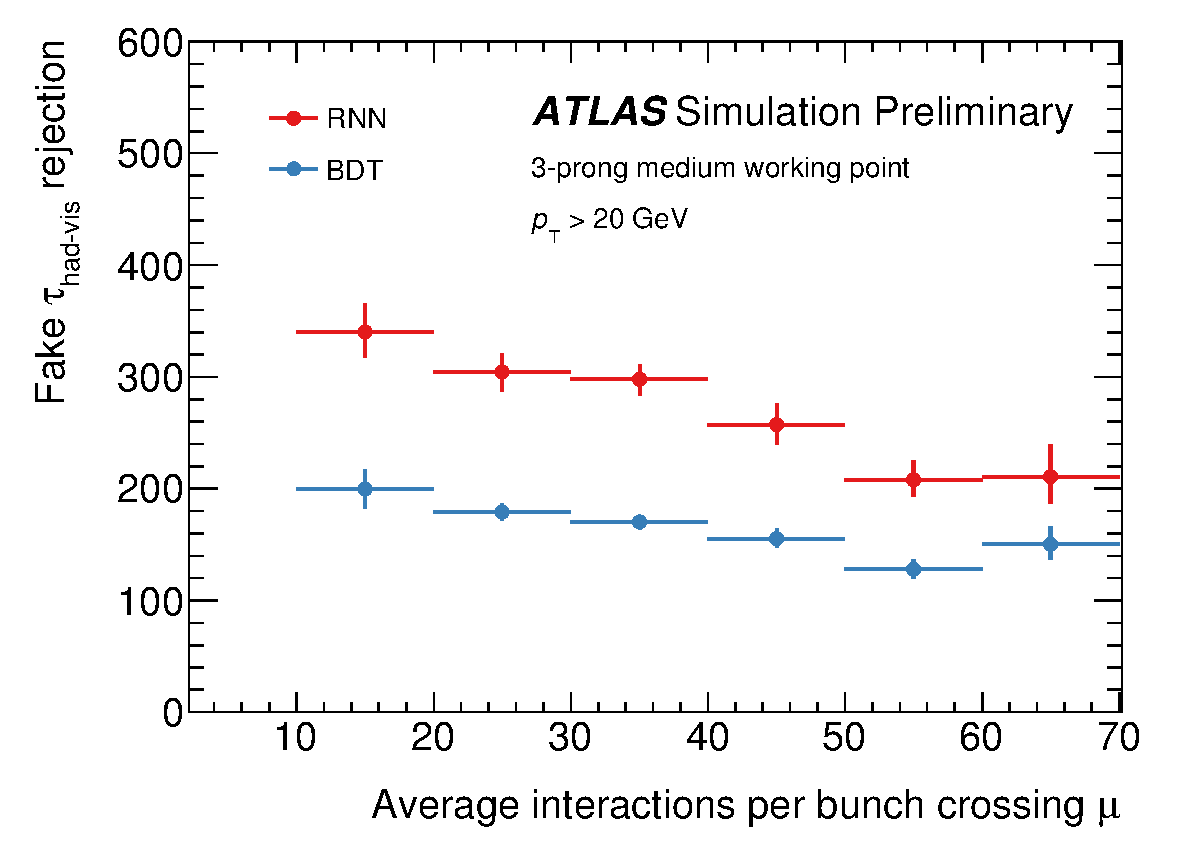
\includegraphics[width=\textwidth]{tauid/pubnote/rej_vs_mu_3p}
    \subcaption{}%
    \label{fig:tauid_faketau_rej_f}
  \end{subfigure}

  \caption[Fake-\tauhadvis rejection of the \emph{medium} RNN and BDT \tauid
  working points.]{Fake-\tauhadvis rejection of the \emph{medium} RNN (red) and
    BDT (blue) \tauid working points. The rejection is shown separately for
    1-prong (left) and 3-prong (right) \tauhadvis candidates in bins of \pT
    (top), $|\eta|$ (middle) of \tauhadvis candidates and the average number of
    interactions per bunch crossing, $\mu$, for the event (bottom). The
    rejection is estimated using a sample of \tauhadvis candidates from
    simulated dijet events. All figures are taken from
    Ref.~\cite{ATL-PHYS-PUB-2019-033}.}%
  \label{fig:tauid_faketau_rej}
\end{figure}

Data-driven measurements of the \tauhadvis identification efficiencies of
selected RNN \tauid working points (\emph{loose}, \emph{medium}, and
\emph{tight}) were performed by the ATLAS collaboration. The measurements used
the tag-and-probe method in $Z \to \tau_\mu \tauhad$ events and have provided
calibrations of the \tauhadvis efficiencies in simulation. A relative agreement
within \SI{5}{\percent} is observed between the efficiency predicted by
simulation and the central value of the data-driven measurement.\footnote{A
  similar level of agreement is observed in the \tauhadvis identification
  efficiency measurements for the BDT-based algorithm.} Both agree within the
statistical and systematic uncertainties of the measurement, showing acceptable
modelling of the \tauid decisions thresholds in simulation even after including
low-level information from charged-particle tracks and topo-clusters.

%%% Local Variables:
%%% mode: latex
%%% TeX-master: "../../phd_thesis"
%%% End:
